\section{Methodology}\label{sec:methodology}
%Hugues
%{\bf BRUNI: je pense que ce qui vient après devrait faire partie de la méthodologie}
%{\bf BRUNI: je trouve que l'idée qui est montrée et développée à la figure 1 est excellente et elle est assez bien développée. Par contre, j'aime beaucoup les paragraphes que j'ai mentionnée sous mon commentaire qui eston dans l'intro...Il faudrait marier les deux, mais je ne sais pas exactement comment. À discuter} 

The method to build the taxonomy presented in this paper was developed to reach the following goals:

\begin{itemize}
\item classify the specific communication applications for ground transportation in terms of categories relevant to the core goals of transport, moving people and goods efficiently, and to its negative impacts, for example crashes and pollution;
\item identify, for each application, other attributes useful for transport, such as the part of the road network and the type of user that is the sole or main focus of each application;
\item identify, for each application, the useful attributes for telecommunications, such as the requirements for proper operation (\acrshort{KPI} requirements) and the implied communication modes (\acrfull{V2I}, \acrfull{V2V}, etc.);
\item list all the current wireless communication technologies, %identify several information in our classification. Just like
  with important attributes such as their performance, their modes of communication or their technologies;% which will have a strong stake in the future. 
\item map the communication technologies that can be used for each transportation application, meeting their \acrshort{KPI} requirements;
\item identify as many applications as possible that may become obsolete with the development of current technologies, especially considering connected and automated vehicles on the one hand and the pervasiveness of smartphones and \acrshort{CT} applications smartphones.
\end{itemize}

The main steps of the method presented in Fig.~\ref{fig:methodology} are described in the following subsections. 

\begin{figure}[ht!]
  \centering
  \begin{tikzpicture}[every text node part/.style={align=center}, scale=1.2]
    \node[label={\small Telecommunication\\ \small Literature},draw,circle,rounded corners=3pt,fill=green!5] (un) at (0,0){\includegraphics[width=.05\textwidth]{arttelecommunication.png}};
         
    \node[label={\small Transportation\\ \small Literature},draw,circle,rounded corners=3pt,fill=blue!5] (deux) at (3,0){\includegraphics[width=.05\textwidth]{arttransport.png}};
    
    \node[label={[xshift=-2.2cm, yshift=-1cm] \small Database},draw,circle,rounded corners=3pt,fill=yellow!5] (trois) at (1.5,-2.3){\includegraphics[width=.05\textwidth]{data.png}};
       
    \node[label={[xshift=-2.2cm, yshift=-1.5cm] \small Information},draw,circle,rounded corners=3pt,fill=white,draw=red] (quatre) at (1.5,-5){\includegraphics[width=.035\textwidth]{t1.png}\includegraphics[width=.035\textwidth]{t4.png}\\
      \includegraphics[width=.035\textwidth]{t5.png}\includegraphics[width=.035\textwidth]{t2.png}\\
      \includegraphics[width=.035\textwidth]{t3.png}\includegraphics[width=.035\textwidth]{t6.png}};
       
    \node[label={[xshift=-2.2cm, yshift=-1cm] \small Taxonomy},draw,circle,rounded corners=3pt,fill=blue!5] (cinq) at (1.5,-8){\includegraphics[width=.05\textwidth]{taxonomy.png}};
       
    \draw[->,draw=green!70!red!50,fill=green!5,line width=0.5mm] (un.south) -- (trois.north west);
    \draw[->,draw=blue!90!black!70,fill=green!5,line width=0.5mm] (deux.south) -- (trois.north east);
    \draw[->,draw=red!70,fill=green!5,line width=0.5mm] (trois.south) -- (quatre.north);
    \draw[->,draw=red!70,fill=green!5,line width=0.5mm] (quatre.south) -- (cinq.north);
  \end{tikzpicture}
  \caption{Methodology overview}
  \label{fig:methodology}
\end{figure}

\subsection{Data Collection}

\subsubsection{Document Search} 

%The data was collected in two steps.
The first step of the data collection was to search for documents, mainly scientific papers in journals and conferences as well as technical reports, in bibliographic databases in the transportation and telecommunication literatures. 
%The various information present in the scientific literature or online were collected according to a predefined route:
%One step was to collect information directly present in the database of Elseiver: Engineering village.
The following concepts and keywords (and synonyms) are taken into account: 

\begin{itemize}
\item Intelligent transportation system (ITS) 
\item Communicating application 
\item Telecommunications and technology (wireless) 
\item Taxonomy and classification
\item Communication system
\end{itemize}

%However, the concepts are not always taken into account in each case.
The following search query was used in Engineering Village\footnote{\url{https://www.engineeringvillage.com/search/quick.url}}: \texttt{(systèmes de transport intelligents OR Intelligent transport* system OR Smart Mobilit*) AND (Application) And (technolog* OR \\ Telecommunication) AND (Vehicular communication systems OR communication platform) AND (Survey OR Taxonomy or Classification)}. This query yielded 279 unique documents, distributed in several databases as indicated in Table~\ref{tab:data_base}.

\begin{table}[ht!]
\centering
\begin{tabular}[ht!]{lc}
\hline
Database \footnote{Result of \url{https://www.engineeringvillage.com/rss/feed.url?queryID=M53259e0417abf827d2fM7ffd127001&SYSTEM_PT=t}} &Number\\
\hline
Compendex &218\\
Inspec &134\\
Knovel &7\\
Duplicates&80\\
\bf {Total}&\bf{279}\\
\hline
\end{tabular}
\caption{Results of the search query per database: Compendex, Inspec and Knovel. } %{\bf NS: ajouter des adresses web?}
\label{tab:data_base}
\end{table}



The results contain several useful documents, including previous taxonomies and classifications that served as the basis to this taxonomy~\cite{papadimitratos_vehicular_2009}. However, this approach does not cover all the potentially useful documents for this research.  %in building the mapping. 
An extra step was to search for reports directly in institutes such as the documents of the European Telecommunications Standards Institute. \cite{etsi_etsi_tr_102_638_intelligent_2009} which have made it possible to standardize a large majority of the names of communicating applications. This report research step is done through our construction of the taxonomy and our personal knowledge. 
Additionally, searches were performed on Google Scholar using keywords such as ``Taxonomy'' or ``Smart Mobility'', which yielded other relevant documents like a taxonomy for planning and designing smart mobility services~\cite{cledou_taxonomy_2018}. Additional searches were done for specific \acrshort{CT} applications on Google Scholar. 
% But for complete information, individual searches by applications or concepts were most often carried out on GoogleScholar. This step consisted of extracting useful information from the papers, synthesizing them and enriching them to build the taxonomy.
Finally, the authors' kowledge and experience from discussions with experts are conferences and meetings were integrated with the information extracted from the documents on specific points. 

\subsubsection{Inclusion Criteria} 

Given the continued and rapid evolution of this field, an important factor for inclusion is the publication date of the documents. The criterion is to consider only documents published less than ten years ago, with some flexibility for slightly older but significant documents.
%However, an older paper may have been taken into account if there was any significance to building applications. 
The second criterion is related to the information in the document. It has to provide useful information related to both fields, transportation and telecommunications, and how telecommunication technologies enable \acrshort{CT} applications. Documents dealing strictly with only one domain were excluded, except for a few documents proposing solid classifications of \acrshort{CT} applications~ \cite{cvria_applications_2016}. 
% As mentioned in the other sections, this taxonomy aims to take into account information useful for telecommunications. Papers dealing only with the purely optical aspect of non-intelligent transport have been excluded. Unless he had a real interest in informing transport entities, such as transport categories  \cite{noauthor_applications_nodate}
Redundant documents were also removed when they did not bring any additional information with respect to documents already included in the set of documents. 
%Exclusion of transport and telecommunications elements unrelated to the construction of the taxonomy on the need for communicating applications and wireless technologies. For example, the studies focus only on communications between two fixed telecommunications structures.
The inclusion or exclusion was decided based on the title of the document, then after reading the abstract, the section titles, figures and tables, and finally the whole document. The final set contains 108~documents. 

\subsection{Overview of the Documents}

\subsubsection{Types of Document}

The documents were classified by type depending on the venue for their publication (conference, journal (or magazine), technical report and online) and by year of publication. As can be seen in Fig.~\ref{fig:type_of_article}. 
%This figure reflects a fairly good representation of the items used in the taxonomy of this study.
most documents were published in journals and magazines which represent about 58~\% of all documents, of which almost 13~\% were published for the year 2017. Then 23~\% of the documents were presented at conferences, 11~\% were publised as technical reports and 7~\% online. However, even though reports constitute a small part of the documents, they provide essential information for our mapping, such as the \acrshort{ETSI} reports~\cite{etsi_etsi_tr_102_638_intelligent_2009,etsi_tr_102_863_intelligent_2011}.
91~\% of the documents meet the criterion on the publication year, i.e.\ were published in the last 10 years (2011 to 2021), including nearly 59~\% between 2014 and 2018. The older documents were collected either for their relevance classifications and taxonomies, or for information missing in more recent literature. 

\begin{figure}[ht!]
  \begin{center}
    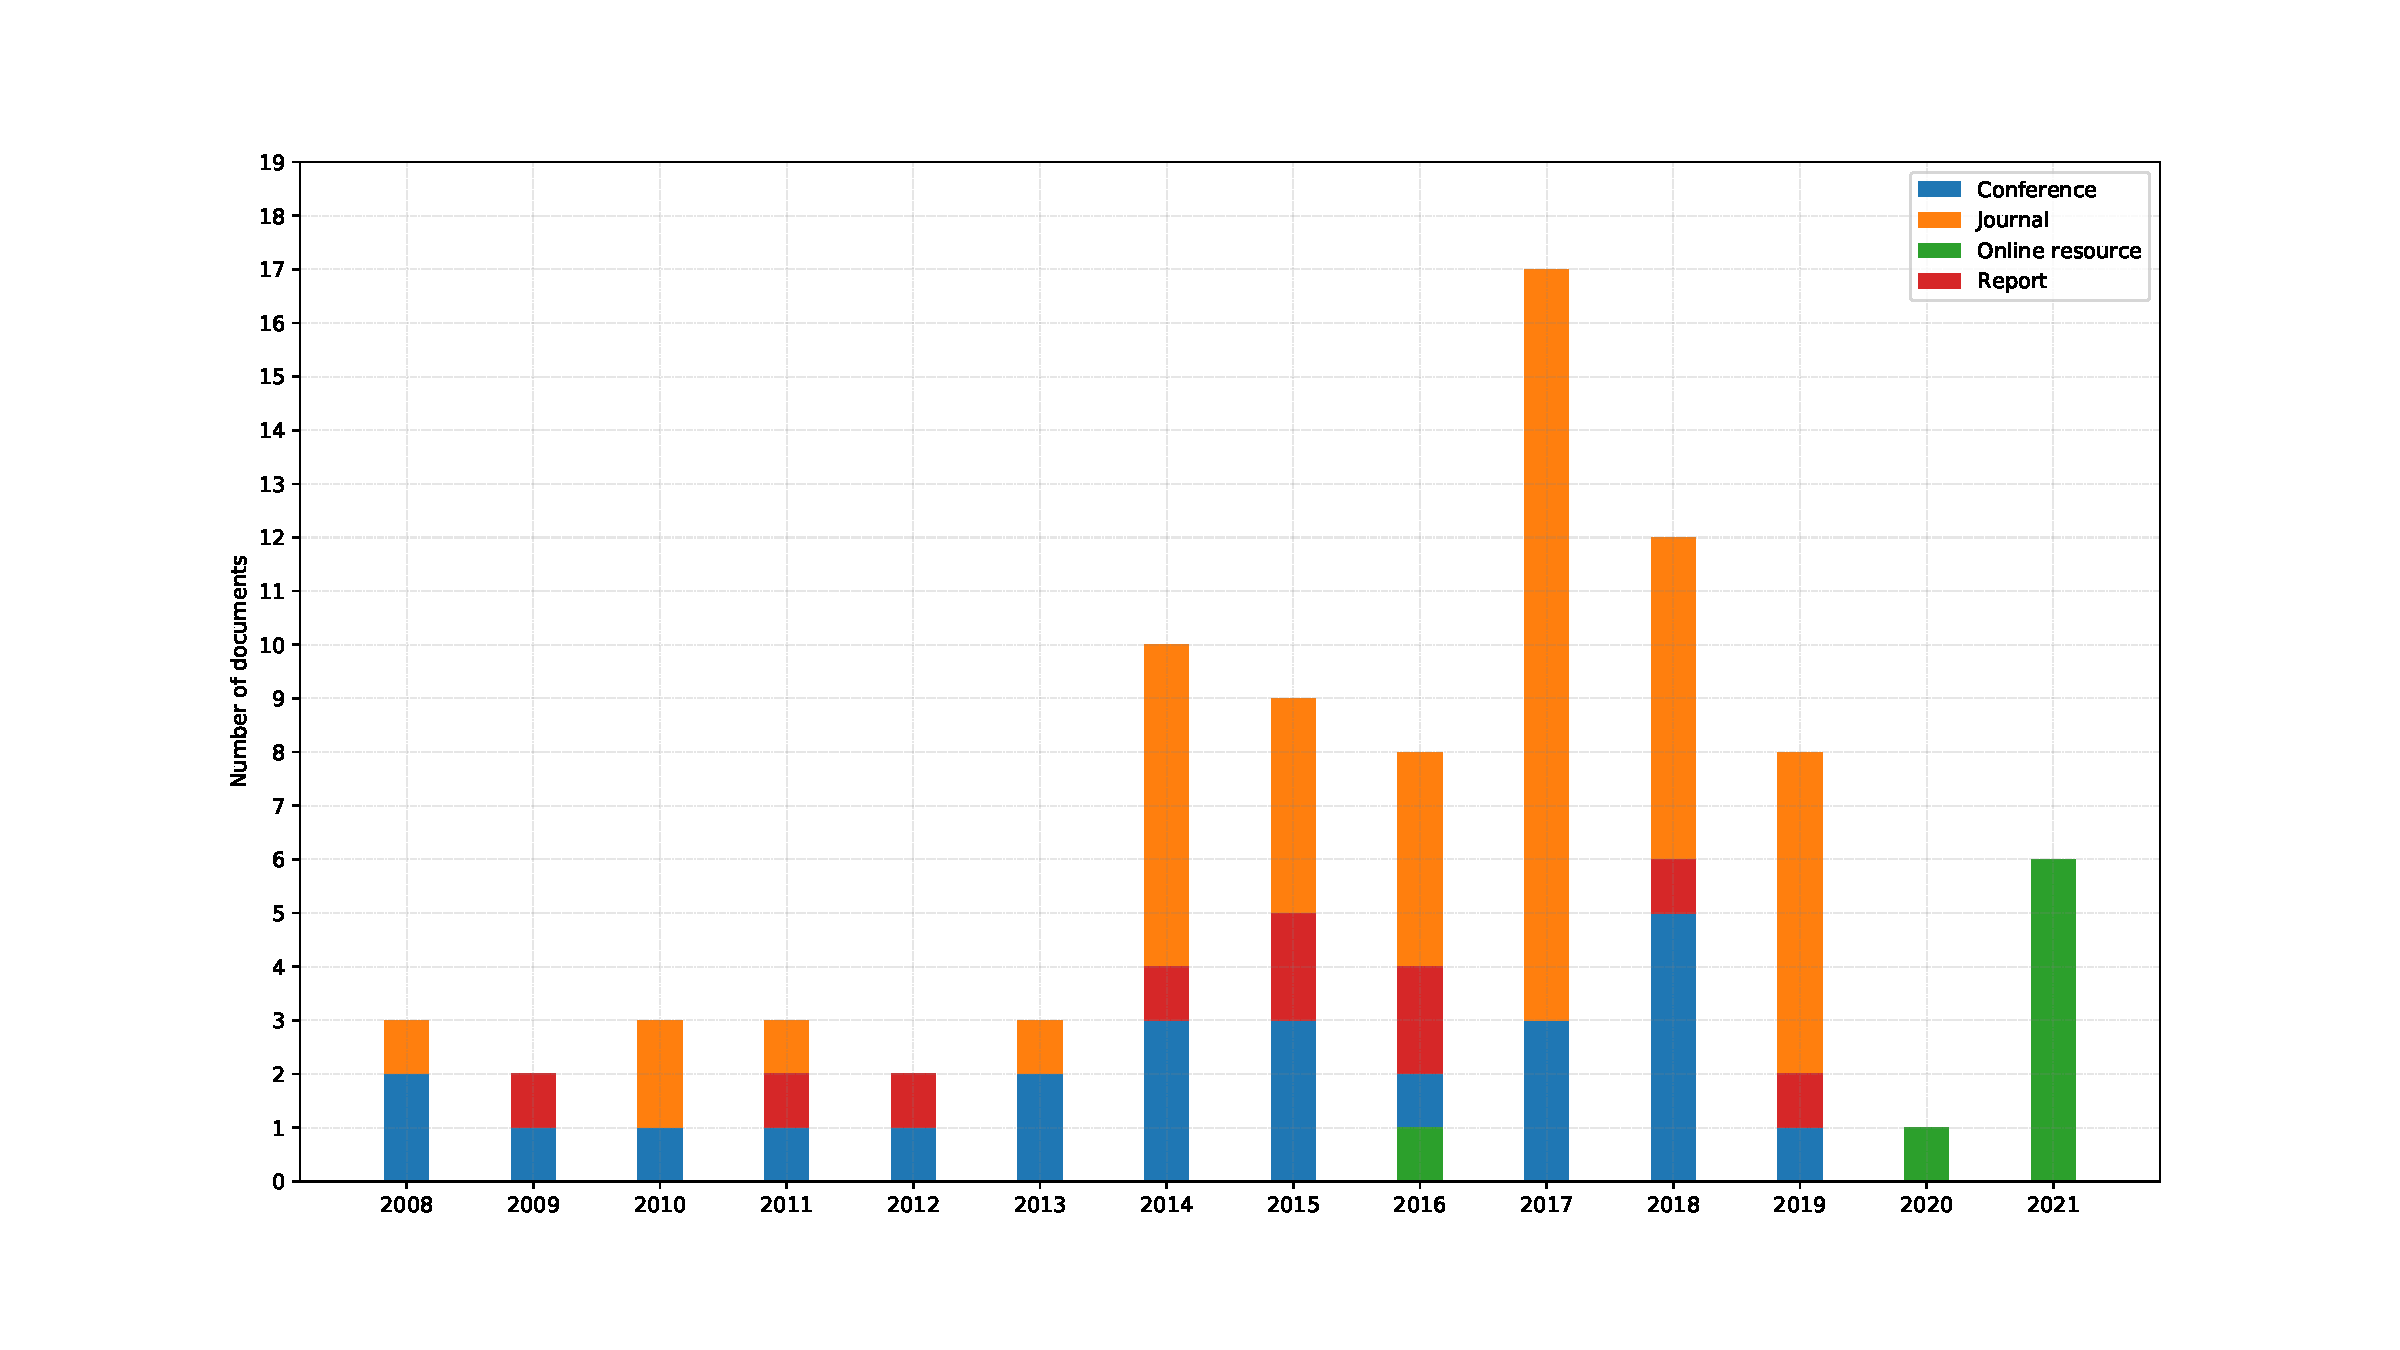
\includegraphics[width=15cm]{document_type.pdf}
    \caption{Number of documents as a function of the year and by type of document (publication venue)}
    \label{fig:type_of_article}
\end{center}
\end{figure}


\begin{table}[ht!]
\centering
\begin{tabular}[ht!]{p{0.04\textwidth}ccccc}
\hline
&Journal&Conference&Report&Online&\bf{Total}\\
\hline
\bf{IEEE}&27&24&-&-&\bf{51}\\
\bf{Elsevier}&14&-&-&-&\bf{14}\\
\bf{MDPI}&8&-&-&-&\bf{8}\\
\bf{USDOT}&-&-&4&5&\bf{9}\\
\bf{Springer}&7&-&-&-&\bf{7}\\
\bf{Other}&7&1&8&3&\bf{19}\\
\hline
\end{tabular}
\caption{Number of documents per publisher (\acrfull{IEEE}; \acrfull{MDPI}; \acrfull{USDOT}). }
\label{tab:publisher}
\end{table}

As the table~\ref{tab:publisher} shows, the main publisher for the documents is the Institute of Electrical and Electronics Engineers (IEEE) with 47~\% of all documents. % This is due to the additional research seen in the previous sections.
As discussed above, starting with the technical reports, in particular by \acrshort{ETSI}, which provided good initial classifications of the \acrshort{CT} applications, additional research for each specific application was done and often lead to papers published in IEEE journals and conference proceedings. One should also note the share of documents (13~\%), mainly scientific papers, published by Elsevier that provided crucial information for the construction of the taxonomy, in particular information from the journal \emph{Transportation Reasearch Part C: Emerging Technologies}

\subsubsection{Document Content}
%The strategy of this research, as mentioned in the previous sections, is to merge the telecommunications information and the transport information. To do this, two steps were taken to collect information from the papers. The first step focused on taxonomies / classifications of applications that allow us to obtain multiple information. With both a wide range of specific applications but also various elements related to telecommunications technologies. The step consisted of a more in-depth or complementary research on the missing information. This information concerns both the specific applications but also the different entities.

The document content was classified in the following categories: 
\begin{itemize}
\item Classification: documents dealing with transportation and/or telecommunication concepts providing a classification of these concepts, instead of a focus on a single entity;
\item Specific Classification: documents dealing providing a classification of transportation and/or telecommunication concepts, focusing on a specific sub-domain instead of attempting a comprehensive classification. An example is a document dealing only with road safety applications.  
\item Specific Application: documents dealing only with a specific \acrshort{CT} application, or a very small number.
\item Specific Technology: documents dealing with a single telecommunication technology, or a very small number. 
\end{itemize}


The resulting classification of the documents is presented in Fig~\ref{fig:information_article}. The documents providing ``general'' classifications and specific classications form the basis for the construction of the taxonomy, about 34~\% of all documents. They usually also provided a lot of information on the different attributes for the \acrshort{CT} applications and communication technologies. Documents on specific applications and technologies let us fill in missing information,
% The fact that specific searches are lower than other types of papers results in very complete information about classification papers, however specific searches have sometimes confirmed certain information of the classification,
for example the \acrshort{KPI}s of wireless telecommunication technologies like 5G.

\begin{figure}[ht!]
  \centering
  % \begin{subfigure}[b]{0.5\textwidth}
  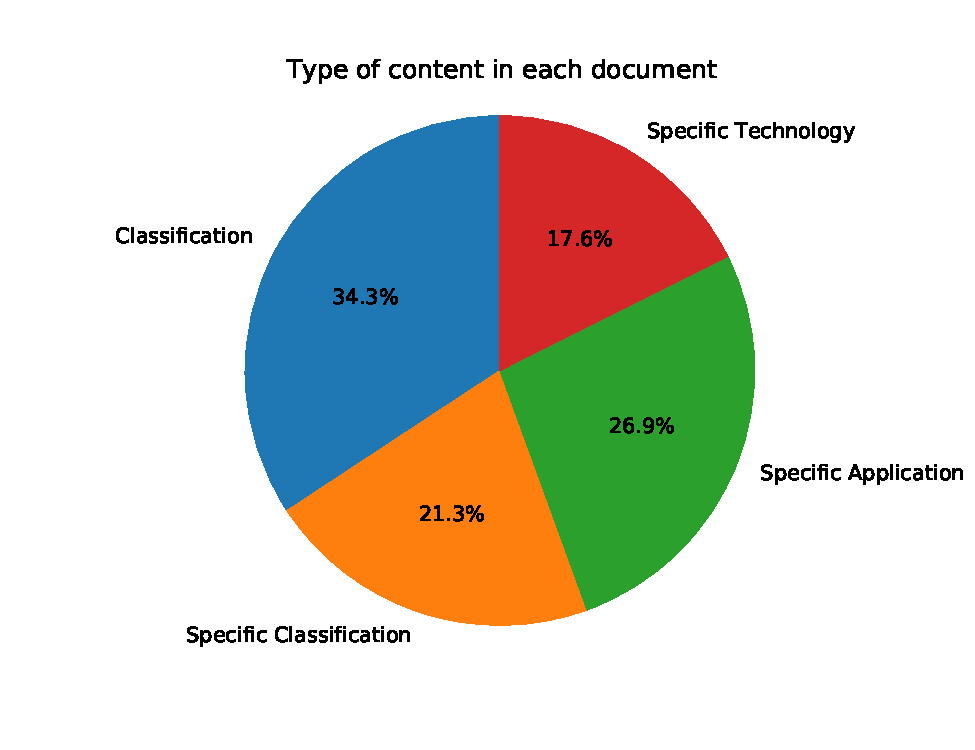
\includegraphics[width=0.33\textwidth]{pie_chart.pdf}
  % \caption{Type of content in each document}
  % \label{fig:pie_chart}
  % \end{subfigure}
\hfill
  % \begin{subfigure}[b]{1\textwidth}
  \includegraphics[width=0.66\textwidth]{information_article.pdf}
  %\caption{Number of documents mentioned each topic.}
  %\label{fig:witouth_ter}
  % \end{subfigure}
\caption{Distribution of the document content (on the left) and proportion of documents mentioning each topic (on the right) }?
    \label{fig:information_article}
\end{figure}



The topics discussed in each document were identified and are presented in Fig.~\ref{fig:information_article}. The most frequent topics are information on specific \acrshort{CT} applications and wireless technologies, which represent respectively 67.5 and 70~\% of the topics covered in the documents. At the other end, topics like the type of road users involved are rarely discussed in the documents (only in 2.78~\%). 
% However, other information which is not very present in the papers but which is very important, such as the types of users were identified in our research,0,7\% .
There are unfortunately fewer documents describing the requirements for each \acrshort{CT} application or the performance of each communicating technologies. These documents are still considered in our set of documents as they may be the only ones to cover a specific application or discuss a new communication technology. 
% Finally, it should be noted that in some papers, specific technologies and applications are discussed, without taking into account the requirement, this type of paper is still necessary for the construction of our taxonomy because it allows both to add additional information but also sometimes to identify technologies not present in the KPI studies . 

\subsection{Taxonomy}
\subsubsection{Definitions}

A taxonomy, originally used in biology, is ``the practice and science of classification of things or concepts'', and also refers to a ``specific classification scheme'' (Wikipedia) \cite{wikipedia_taxonomy_2021}
% More precisely, it is a science of classification that is widespread
It has become synonymous with classification and quite common in all scientific and technical fields. This makes it possible to group together concepts or objects. The goal of this paper is to classify \acrshort{CT} applications both in terms of abstract concepts like transportation application categories (e.g., safety) and of objects like communication technologies. 

\subsubsection{Taxonomy construction}

The taxonomy was build in three main steps. The first step started with the transportation field and the study of \acrshort{CT} applications. The area(s) or categorie(s) and other attributes of each application were identified and similar applications were grouped together. This resulted in a list of areas and attributes that were chosen based on the literature and our understanding of the applications. 
%More precisely that we group the applications according to transport criteria. This can be groupings in terms of "definition", for example two applications are close to transport safety applications. But we will also take into account other classification criteria such as types of users, type of roads, etc. 
The second step consisted in studying the \acrshort{CT} applications in the context of telecommunication technologies. The requirements and mode of communication (e.g.\ \acrshort{V2V} and/or \acrshort{V2I}) of each application to enable their proper implementation were researched. On the other side, the corresponding performance and attributes of current communication technologies were also documented. 
The last step was to match or map the two fields, in order to identify the possible communication technologies for each \acrshort{CT} application based on their respective performance and requirements. The results can be investigated in several ways, for example to study the requirements and suitable communicationt technologies by transportation categories. 
%the class to which it belongs and what technologies can be used for the proper implementation of these applications. But also by looking at other criteria such as the articulation of each transport class of representative KPIs.  This point is one of the innovative features that this paper brings to transport classifications. 

\subsubsection{Representation}
There is no one way to represent a taxonomy, especially this taxonomy as it connects two differents fields, and the attributes and their relationships are complex.
Multiple representations can be used, for example hierarchical representation like trees for 1 to $n$ associations, or graphical representations like Sankey diagrams for more general $m$ to $n$ associations. The choice depends on the goal of the representation and how it can be interpreted. 
%In our case, as we will see in the result part, we will take a large number of representations according to the chosen concepts. This can range from tables to Sankey for transportation categories. 

%This part is all the more important as it allows to have credible arguments on the chosen classification but also to make the classification visible to the reader. 

The most important representations are presented as tables and figures in this paper. The information about the documents, \acrshort{CT} applications and communication technologies gathered in this project is shared on a public GitHub repository~\url{https://github.com/HuguesBlache/taxonomy}, along with Jupyter notebooks containing the Python code to generate the figures presented in this paper. This repository contains other figures, as well as interactive visualizations (charts) using the plotly library that can be run on the binder platform \url{https://mybinder.org/}. Sharing the data and the code used to produce the results presented in this paper allows other researchers to build upon this work. 

% \paragraph{Visualisation}

% The graphics in this paper were built on a Jupyter-NoteBook using extensively the Plotly scientific graphics libraries. One of the advantages of these charts is that most of the charts and tables you create are interactive. 

% \paragraph{Interactive}

% To give a more dynamic reading to the reader, all the programs, which made it possible to directly construct the figures, were compiled in mybinder and depedantes of the database. For more explanations, a GitHub has been built in open access:  HuguesBlache/Taxonomy
 

